\section{Numerical Simulations}

\subsection{Environmental flux}

SPENVIS uses the AP-8/AE-8 model to simulate the trapped proton and electron models, which can simulate the fluxes during solar maximum and minimum.

For the worst-case simulation the solar maximum is considered. 

For the protons the number of trapped protons is higher during solar minimum due to the increased scale height caused by the increased UV radiation from the sun, but only for lower altitudes, for this orbit the difference between solar minimum and maximum for the proton flux is negligible, which is not the case for the electrons.

In figures \ref{fig:e_map} and \ref{fig:p_map} the integrated fluxes are displayed over the orbit in GEI mode.

The highes proton fluxes are expected at perigee, while for the electron flux the highes flux is expected during crossing of the radiation belts (c.f. fig. \ref{fig:e_wmap}).

\begin{figure}[!htbp]
  \centering
  \begin{minipage}[b]{0.45\textwidth}
    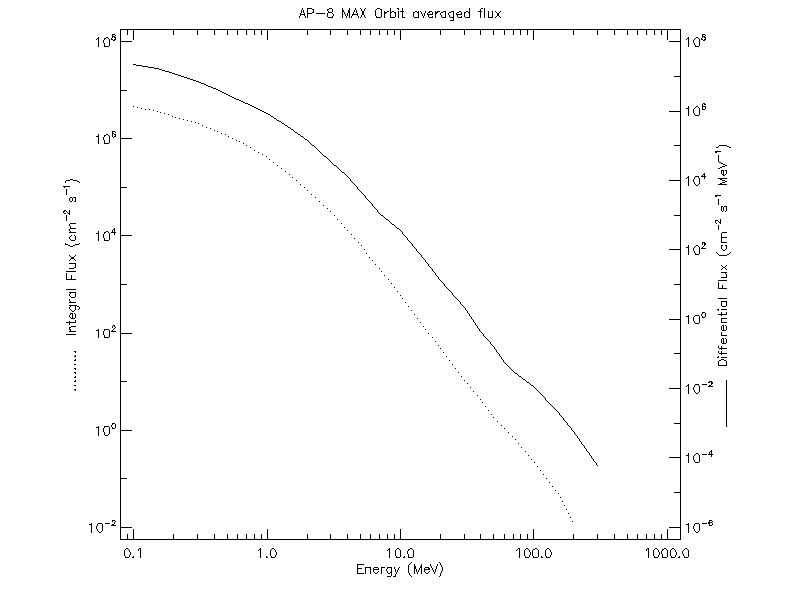
\includegraphics[width=\textwidth]{spenvis/max_prot}
    \caption{Proton Flux}
    \label{fig:p_flux}
  \end{minipage}
  \hfill
  \begin{minipage}[b]{0.45\textwidth}
    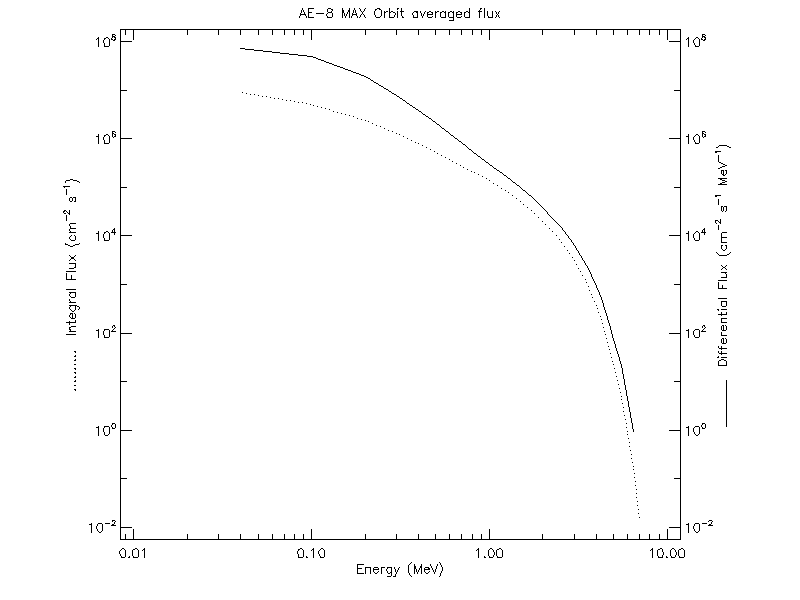
\includegraphics[width=\textwidth]{spenvis/max_elec}
    \caption{Electron Flux}
    \label{fig:e_flux}
  \end{minipage}
\end{figure}

\begin{figure}[!htbp]
  \centering
  \begin{minipage}[b]{0.45\textwidth}
    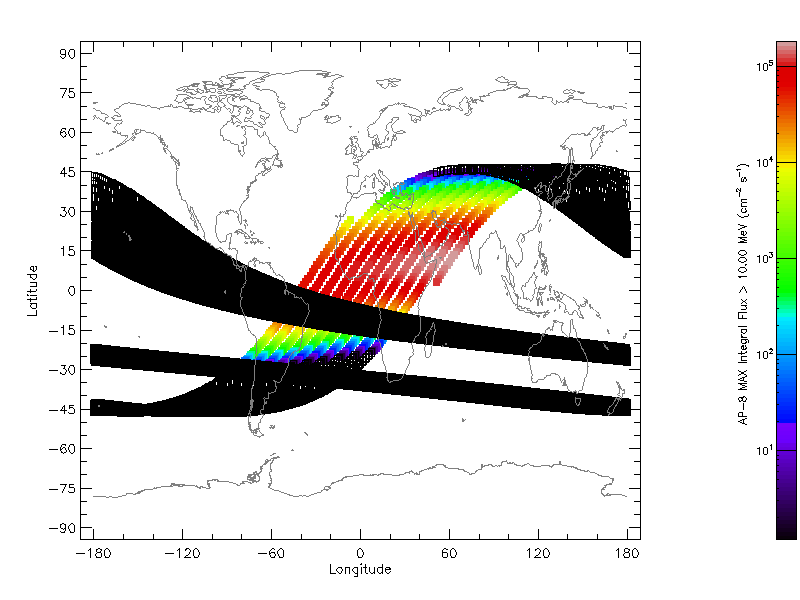
\includegraphics[width=\textwidth]{spenvis/proton_map}
    \caption{Proton Flux greater than 1 MeV}
    \label{fig:p_map}
  \end{minipage}
  \hfill
  \begin{minipage}[b]{0.45\textwidth}
    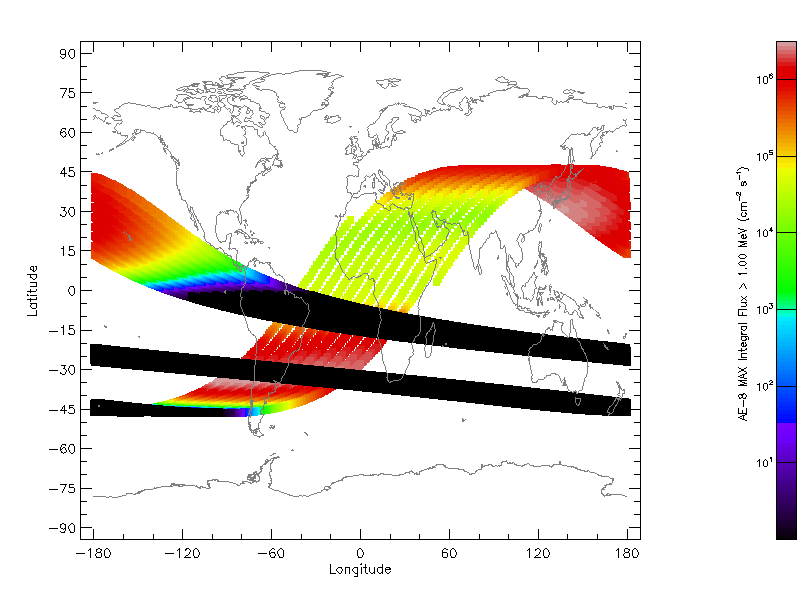
\includegraphics[width=\textwidth]{spenvis/electron_map}
    \caption{Electron Flux greater than 1 MeV}
    \label{fig:e_map}
  \end{minipage}
\end{figure}

\begin{figure}[!htbp]
	\centering
	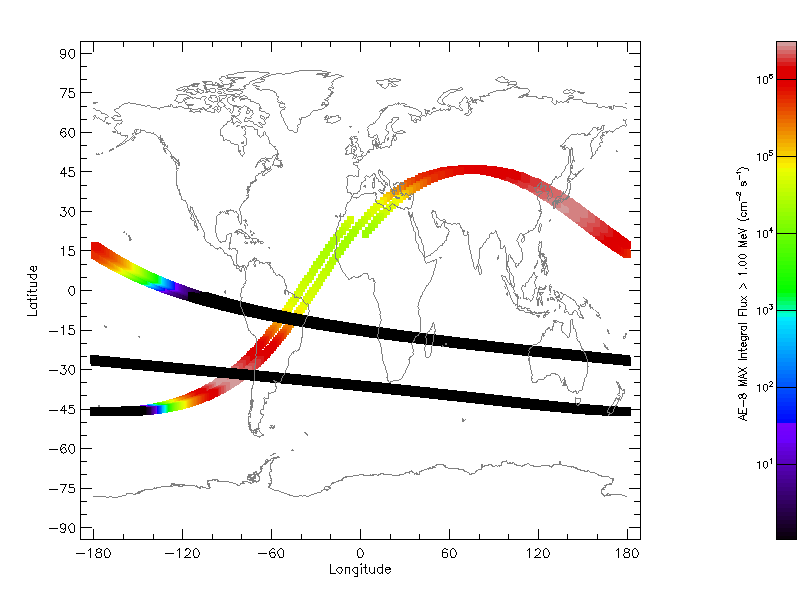
\includegraphics[width=.5\linewidth]{spenvis/electron_wmap}
		\caption{Electron Flux World map}
		 \label{fig:e_wmap}
\end{figure}

\subsection{Lifetime and Performance Degradation}

The satellite is using Azur 3G28 solar cells, with an EOL power of 95\% of the BOL power \citep{evans:labInstructions}.

Using SPENVIS' MC-SCREAM for solar cells, it was determined that the shielding thickness should be around 230 \textmu m which leaves an EOL powerloss of 3.3\%.

\subsection{Total Dose and Shielding}

The satellite is using a memory device which can withstand a total radiation dose of 25 Krad before failure.

With 1mm of shielding the memory device exceeds its maximum radiation dose with a total dose of 1.5 Mrad, which is about 62 times the maximum allowed dose.

To achieve a maximum dose of 25 Krad or less the shielding has to be increased to a minimum of 5.1mm, which will lead to a maximum dose of 26 Krad.

\begin{figure}[!htbp]
	\centering
	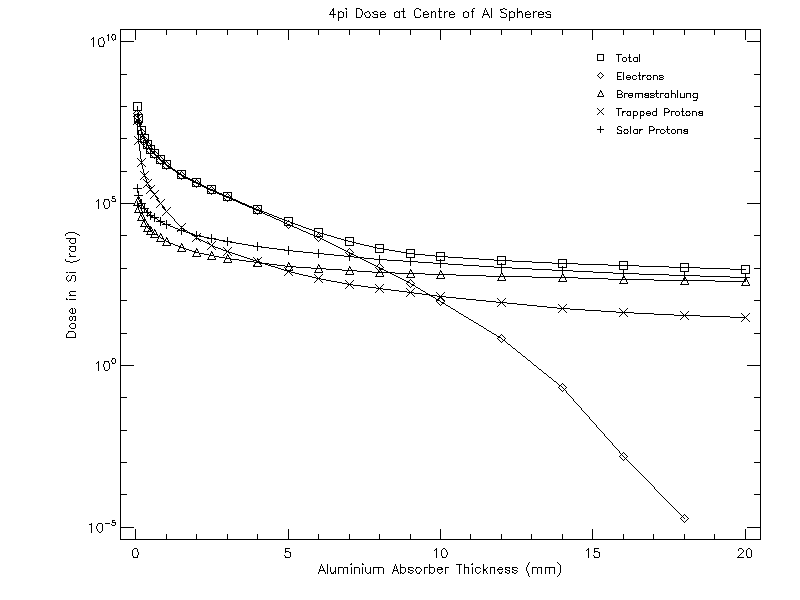
\includegraphics[width=.5\linewidth]{spenvis/memory_rad}
		\caption{Dose received vs. Shielding in mm}
		 \label{fig:rad_memory}
\end{figure}
\subsection{Single Event Upsets}

\subsubsection{Linear Energy Transfer (LET) Spectrum}

The LET spectra was calculated using SPENVIS, including solar particles, trapped protons and galactic cosmic rays, with a shielding of 1 $g/cm^2$ (c.f. fig. \ref{fig:let_spectra}).

\begin{figure}[!htbp]
	\centering
	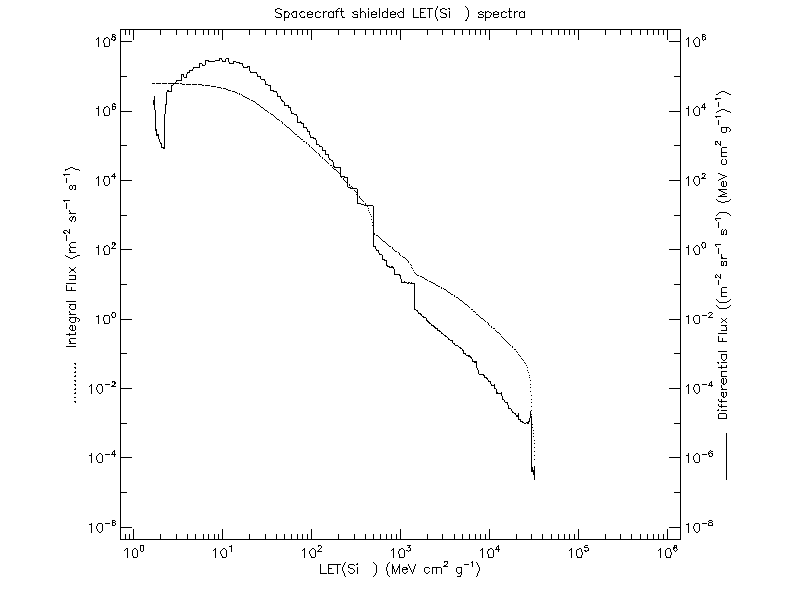
\includegraphics[width=.5\linewidth]{spenvis/LET_spectra}
		\caption{LET spectra for the full mission}
		 \label{fig:let_spectra}
\end{figure}

\subsubsection{Cross Section and Components Characteristics}

For the SEU estimation several parameters are needed for the SMJ329C50GFAM66 to determine its cross-section which is determined by a Weibull function.

\begin{equation*}
\sigma(L) = \begin{cases}
0 &\text{$L \geq L_0$}\\
C_s \left ( 1 - e^{\left (\frac{L-L_0}{W}  \right )^{s} } \right ) &\text{$L < L_0$}
\end{cases}
\label{eqn:weibull}
\end{equation*}

Using the mono-beam experimental results (\citep{evans:labInstructions}) the final parameters calculated with a Weibull-fit in Matlab are:
\begin{table}[!htp]
 \centering
 \begin{tabular}{lr}
  $L_0$ & $1.01 MeV\cdot cm² / mg$  & LET Threshold\\
  $C_s$ & $4.985 10^{-6} cm²$  & saturated crosssection\\
  $W$ & $4.985 MeV\cdot cm² / mg$  & Weight of the distribution\\
  $s$ & $0.7$  & shape parameter\\
 \end{tabular}
 \label{table:weibull}
 \caption{Results of the Weibull-Fit}
 \end{table}
 
 The code responsible for the fit is generated using the Matlab Curve-Fit Toolbox (c.f. Listing \ref{code:fit}) using data from \citep{evans:labInstructions} (c.f. Listing \ref{code:fit_values}).
 
 \begin{center}
\begin{lstlisting}[language=Matlab,caption={Autogenerated Matlabcode for fitting},label=code:fit]

function [fitresult, gof] = createFit(stopping, crossSec)
%CREATEFIT(STOPPING,CROSSSEC)
%  Create a fit.
%
%  Data for 'Weibull' fit:
%      X Input : stopping
%      Y Output: crossSec
%  Output:
%      fitresult : a fit object representing the fit.
%      gof : structure with goodness-of fit info.
%
%  See also FIT, CFIT, SFIT.

%  Auto-generated by MATLAB on 27-Mar-2016 22:16:28

[xData, yData] = prepareCurveData( stopping, crossSec );

% Set up fittype and options.
ft = fittype( 'C*(1-exp(-((x-L)/w)^s))', 'independent', 'x', 'dependent', 'y' );
opts = fitoptions( 'Method', 'NonlinearLeastSquares' );
opts.Display = 'Off';
opts.StartPoint = [0.0003 1 1 2];

% Fit model to data.
[fitresult, gof] = fit( xData, yData, ft, opts );
\end{lstlisting} 
 \end{center} 


 \begin{center}
\begin{lstlisting}[language=Matlab,caption={Inputvalues for the fit},label=code:fit_values]
flips =[8 7497 22514 23986 33810 29991 21022 18043]; %from instructions
exTime = [5 5 5 5 5 10 10 15]; %from instructions
flux = [25e6 25e6 25e6 17e6 23e6 10e6 7e6 4e6]; %from instructions
energyBeam = [0.6 0.72 9.6 4.8 20 56 84 786]; %from instructions
u = [12 12 12 16 40 56 84 131]; %from instructions
energy = energyBeam./(u); %Where it has to be read from the table
crossSec=flips./(exTime.*60.*flux); %crosssection
LET = [2.73E+03 3.13E+03 4.65E+03 7.23E+03 1.77E+04 2.77E+04 3.74E+04 5.72E+04]./1000; %MEV cm^2/mg, read from table
\end{lstlisting} 
 \end{center} 

\subsubsection{SEU Estimation}

To determine which device is best for the mission it is neccessary which possible device is most immune to radiation to minimize malicious operation or data corruption.

This is done by estimating the SEU (single-event upset).

The SEU is calculated with the following formula (assuming omnidirectional flux), which was done using the results from the SPENVIS simulation in Matlab.

\begin{equation*}
\frac{dU}{dt} = 4 \pi \int_{0}^{\infty} \sigma\left ( LET \right ) \sum_{z=92}^{z=0}h\left ( LET \right )dLET
\end{equation*}